\documentclass[pt12]{beamer}
%\documentclass[pt12,externalviewer]{beamer}

\usepackage{amssymb}
%\usepackage{rotating}
%\usepackage{amsmath}
\usepackage{tikz}
\usetikzlibrary{patterns} % Add this line to use patterns
%\usepackage{beamergraphics}
\usepackage[english]{babel}
\usepackage[latin1]{inputenc}
\usepackage[T1]{fontenc}
\usepackage{cleveref}
\usepackage{nicematrix}
\usepackage{mathptmx}
\usepackage{anyfontsize}
\usepackage{t1enc}
\usepackage{pgfmath}

%\usepackage[absolute,overlay]{textpos}
%\usepackage{pdfcolparallel}

\usepackage{tcolorbox}
%\tcbuselibrary{fitting}
\usepackage{mdframed}

\usepackage{lipsum}

\usepackage{adjustbox}

%\usepackage{subfig}
\usepackage{caption}
\usepackage{subcaption}
\usepackage{pgfplots}
\pgfplotsset{width=7.5cm,compat=1.12}
\usepgfplotslibrary{fillbetween}
\usepackage{media9}

\definecolor{BBB}{rgb}{0.2,0.2,0.7} % UBC Blue (primary)
\definecolor{SSCgreen}{HTML}{a2da7b} % green as in the SSC logo (primary)
\definecolor{SSCdarkgreen}{HTML}{437024}
\definecolor{SSCred}{HTML}{d5685d}   % red   as in the SSC logo (primary)
\definecolor{SSCdarkred}{HTML}{bf2413}

%\usebackgroundtemplate%
%{%
%    \begin{tikzpicture}
%      \hspace{3truecm}\node[opacity=0.4] at (0,0) 
%        {\includegraphics[width=\textwidth]{sscback.pdf}};
%    \end{tikzpicture}
%}

\mode<presentation>
{
%  \usetheme{Warsaw} 
  \usetheme{Madrid}
%  \usetheme{Montpellier}
%  \usetheme{Marburg} 
  \usecolortheme[named=BBB]{structure}
  \setbeamercolor{alerted text}{fg=SSCdarkred}
  \setbeamercovered{transparent}
  \setbeamertemplate{section in toc}[ball unnumbered]
}

%\setbeamertemplate{footline}{\hfill\insertframenumber/\inserttotalframenumber} 

\expandafter\def\expandafter\insertshorttitle\expandafter{%
  \insertshorttitle\hfill%
  \insertframenumber\,/\,\inserttotalframenumber}






%\usetikzlibrary{fit}
\usetikzlibrary{arrows}
\usetikzlibrary{trees}


\tikzstyle{bag} = [text width=8em,
text centered]

\tikzstyle{bag_mod} = [text width=2em,
text centered]

\tikzstyle{bag_rect} = [draw=black,rectangle, black,text width=8em,
text centered]

\tikzstyle{bag1} = [draw=black,rectangle, black,text width=4em,
text centered]


\setbeamercolor{blockcolor1}{fg=black,bg=bluemathlab!10}
\setbeamercolor{blockcolor2}{fg=black,bg=orangemathlab!10} 

\definecolor{bluemathlab}{HTML}{065895}
\definecolor{orangemathlab}{HTML}{F79A25}
\colorlet{bluemathlab_alpha}{bluemathlab!70!white}
\colorlet{orangemathlab_alpha}{orangemathlab!70!white}


\newcommand{\Cross}{$\mathbin{\tikz [x=1.4ex,y=1.4ex,line width=.2ex, red] \draw (0,0) -- (1,1) (0,1) -- (1,0);}$}%
\def\L{\mathcal{L}}
\def\I{\mathcal{I}}
\def\R{\mathbb{R}}
\def\bbc{\underline{\boldsymbol{c}}}
\def\bc{\boldsymbol{c}}
\def\br{\boldsymbol{r}}
\def\bd{\mathbf{d}}
\def\bbd{\underline{\mathbf{d}}}
\def\bphi{\underline{\phi}}
\def\M{\underline{\underline{\mathrm{M}}}}
\newcommand{\mass}{\mathbb M}

\newcommand{\Prod}{p}
\newcommand{\dest}{d}
\newcommand{\Ip}{\mathcal{I}}
\newcommand{\bby}{\mathbf{y}}
\newcommand{\highlight}[1]{\textbf{\color{bluemathlab}#1}}
\newcommand{\highlightB}[1]{\textbf{\color{black!15!orangemathlab}#1}}
\newcommand{\mathhighlight}[1]{\color{bluemathlab}#1}
\newcommand{\mathhighlightB}[1]{\color{black!15!orangemathlab}#1}



\newcommand{\backupbegin}{
   \newcounter{framenumberappendix}
   \setcounter{framenumberappendix}{\value{framenumber}}
}
\newcommand{\backupend}{
   \addtocounter{framenumberappendix}{-\value{framenumber}}
   \addtocounter{framenumber}{\value{framenumberappendix}} 
}

\newcommand{\refer}[1]{%
   \begin{flushright}
      {\alert{\tiny #1}}
   \end{flushright}}
  
\newcommand{\lrefer}[1]{%
   \begin{flushleft}
      {\alert{\tiny #1}}
   \end{flushleft}}
  
\newcommand{\param}[1]{%
   \begin{flushright}
      {\small #1}
   \end{flushright}
   \vspace{-1.5\baselineskip}
}

\newcommand{\sech}{\mathop{\rm sech}\nolimits}
\newcommand{\sgn}{\mathop{\rm sgn}\nolimits}
\newcommand{\etal}{{\em et al.}}


\newtheorem{observation}{Observation}
\newtheorem{proposition}{Proposition}
\newtheorem{cor}{Corollary}

\newcommand{\prob}[0]{P}

\newcommand{\lop}[0]{\mathcal{L}}
\newcommand{\lopd}[0]{\mathcal{L}_\Delta}
\newcommand{\lopdt}[0]{\mathcal{L}_{\Delta}}
\newcommand{\usol}[0]{\underline{\uvec{u}}_\Delta}
\newcommand{\usoldt}[0]{\underline{\uvec{u}}_\Delta}

\newcommand{\uex}[0]{\underline{\uvec{u}}^{ex}}
\newcommand{\up}[0]{\underline{\uvec{u}}^{(p)}}

\newcommand{\usoldto}[0]{\tilde{\underline{\uvec{u}}}_\Delta}

\newcommand{\uapp}[0]{\uvec{u}_h}
\newcommand{\wapp}[0]{w_h}

\newcommand{\massmatrix}[0]{\mathcal{M}}

\newcommand{\tess}[0]{\mathcal{T}_h}


%\newcommand{\uvec}[2][3]{\underline{#2\mkern-#1mu}\mkern#1mu}
%\newcommand{\uvec}[2][3]{\mathbf{#2\mkern-#1mu}\mkern#1mu}
\newcommand{\uvec}[2][3]{\boldsymbol{#2\mkern-#1mu}\mkern#1mu}


\newcommand{\res}[0]{\textbf{R}}
\newcommand\norm[1]{\left\lVert#1\right\rVert}

\newcommand{\flux}[0]{\boldsymbol{f}}
\newcommand{\source}[0]{\boldsymbol{S}}
\newcommand{\ST}[0]{\boldsymbol{ST}_i^K}
\newcommand{\extra}[0]{\boldsymbol{ST}_i}


\newcommand{\elres}[0]{\uvec{\Phi}^K(\uapp)}
\newcommand{\noderes}[0]{\uvec{\Phi}^K_i(\uapp)}

\newcommand{\spacestuff}[0]{\boldsymbol{\phi}_i}

\newcommand{\cund}[0]{\underline{\uvec{c}}}

\newcommand{\lopdi}[0]{\mathcal{L}_{\Delta,i}}

\newcommand{\csoldt}[0]{\underline{\uvec{c}}_\Delta}

\newcommand{\basis}[0]{\uvec{v}}


%%%%%%%
\newcommand{\dpar}[2]{\dfrac{\partial #1}{\partial #2}}
\newcommand{\bu}{\mathbf{u}}
\newcommand{\bv}{\mathbf{v}}
\newcommand{\Bv}{\underline{\mathbf{v}}}
\newcommand{\bbv}{\mathbf{v}}
\newcommand{\Bbv}{\underline{\mathbf{v}}}
\newcommand{\bF}{\mathbf{F}}
\newcommand{\bG}{\mathbf{G}}
\newcommand{\bbS}{\mathbf{S}}
\newcommand{\bFF}{\mathcal{F}}
\newcommand{\bbF}{\mathbf{\mathcal{F}}}
\newcommand{\bK}{\mathbf{K}}
\newcommand{\bbu}{\mathbf{u}}
\newcommand{\bbg}{\mathbf{g}}
\newcommand{\hbbg}{\hat{\mathbf{g}}}
\newcommand{\hbbf}{\hat{\mathbf{f}}}
\newcommand{\hbbU}{\hat{\mathbf{U}}}
\newcommand{\hbbfe}{\hat{\mathbf{f}}_{\sigma,\sigma'}}
\newcommand{\ba}{\mathbf{a}}
\newcommand{\bx}{\mathbf{x}}
\newcommand{\by}{\mathbf{y}}
\newcommand{\red}[1]{\textcolor{red}{#1}}
\newcommand{\blue}[1]{\textcolor{blue}{#1}}
\newcommand{\ICI}{\red{\large{ICI}}}

% ---- Notation Philipp
\newcommand{\ww}[1]{\underline{#1}}
\renewcommand{\div}{\operatorname{div}}
\newcommand{\est}[1]{\left\langle#1\right\rangle}
\newcommand{\bU}{\mathbf{U}}
\newcommand{\bH}{\mathbf{H}}
\newcommand{\dd}{\mathrm{d}}
\newcommand{\bV}{\mathbf{V}}
\newcommand{\mean}[1]{\overline{#1}}
\newcommand{\bbfh}{{\mathbf {f}^h}}
\newcommand{\Ol}{\mathcal{O}}
\newcommand{\WW}{\mathrm{W}}
\newcommand{\LL}{\mathcal{L}}
\newcommand{\II}{\hat{I}_0}
\newcommand{\1}{\begin{pmatrix}
		1\\
		1
\end{pmatrix}}
\newcommand{\e}[1]{\mathrm{e^{#1}}}
\newcommand{\VV}{\mathcal{V}}

\newcommand{\CU}{\mathcal{U}}

\newcommand{\iip}{i+1/2}
\newcommand{\iin}{i-1/2}

\newcommand{\jjp}{j+1/2}
\newcommand{\jjn}{j-1/2}

%Dante
\newcommand{\diff}[1]{{\mathrm{d}{#1}}}
\newcommand{\dotprod}{\boldsymbol \cdot}
\newcommand{\ddt}[1]   {\frac{\partial{#1}}{\partial{t}}}
\newcommand{\ddx}[1]   {\frac{\partial{#1}}{\partial{x}}}
\newcommand{\ddy}[1]   {\frac{\partial{#1}}{\partial{y}}}
\newcommand{\dsddt}[1] {\dfrac{\partial{#1}}{\partial{t}}}
\newcommand{\txddt}[1] {\tfrac{\partial{#1}}{\partial{t}}}
\newcommand{\ddp}[2]   { \frac{\partial #1}{\partial #2}}
\newcommand{\dsddp}[2] {\dfrac{\partial #1}{\partial #2}}
\newcommand{\txddp}[2] {\tfrac{\partial #1}{\partial #2}}
\newcommand{\ddo}[2]   { \frac{\diff #1}{\diff #2}}
\newcommand{\dsdo}[2]  {\dfrac{\diff #1}{\diff #2}}
\newcommand{\txddo}[2] {\tfrac{\diff #1}{\diff #2}}
\newcommand{\Div}[1] { \boldsymbol{\nabla} \!\dotprod #1 }
\newcommand{\Grad}[1] { \boldsymbol{\nabla} #1 }
\newcommand{\Gradr}[1]{\widetilde{\boldsymbol{\nabla} {#1}}}
\newcommand{\vect}[1] {\ww{#1}}
\newcommand{\versor}[1] {\hat{ \boldsymbol{#1}}}
\newcommand{\vzero}{\boldsymbol{0}}
\newcommand{\IdxM} {\mathbb{I}}
%%%%%%%


\newcommand{\mysetminusD}{\hbox{\tikz{\draw[line width=0.6pt,line cap=round] (3pt,0) -- (0,6pt);}}}
\newcommand{\mysetminusT}{\mysetminusD}
\newcommand{\mysetminusS}{\hbox{\tikz{\draw[line width=0.45pt,line cap=round] (2pt,0) -- (0,4pt);}}}
\newcommand{\mysetminusSS}{\hbox{\tikz{\draw[line width=0.4pt,line cap=round] (1.5pt,0) -- (0,3pt);}}}

\newcommand{\mysetminus}{\mathbin{\mathchoice{\mysetminusD}{\mysetminusT}{\mysetminusS}{\mysetminusSS}}}




%Numerical schemes
\newcommand{\xip}{x_{i+1/2}}
\newcommand{\xin}{x_{i-1/2}}

\newcommand{\yjp}{y_{j+1/2}}
\newcommand{\yjn}{y_{j-1/2}}




\newcommand{\B}{\widetilde{B}}
\newcommand{\C}{\widetilde{C}}
\newcommand{\Ubar}{\overline{\uvec{U}}}
\newcommand{\Vbar}{\overline{\uvec{V}}}

\newcommand{\FtildeNum}{\widehat{\widetilde{\uvec{F}}}}
\newcommand{\GtildeNum}{\widehat{\widetilde{\uvec{G}}}}
%\newcommand{\FtildeNum}{\uvec{\widetilde{{\cal F}}}}
%\newcommand{\GtildeNum}{\uvec{\widetilde{{\cal G}}}}


%\newcommand{\Bnonbald}[2]{\widetilde{#1}^#2}
%\newcommand{\Bbald}[2]{\widetilde{\uvec{#1}}^#2}
\newcommand{\Bnonbald}[2]{\widetilde{#1}}
\newcommand{\Bbald}[2]{\widetilde{\uvec{#1}}}


\def\restriction#1#2{\mathchoice
              {\setbox1\hbox{${\displaystyle #1}_{\scriptstyle #2}$}
              \restrictionaux{#1}{#2}}
              {\setbox1\hbox{${\textstyle #1}_{\scriptstyle #2}$}
              \restrictionaux{#1}{#2}}
              {\setbox1\hbox{${\scriptstyle #1}_{\scriptscriptstyle #2}$}
              \restrictionaux{#1}{#2}}
              {\setbox1\hbox{${\scriptscriptstyle #1}_{\scriptscriptstyle #2}$}
              \restrictionaux{#1}{#2}}}
\def\restrictionaux#1#2{{#1\,\smash{\vrule height .8\ht1 depth .85\dp1}}_{\,#2}} 



\title[]{\textcolor{white}{\bfseries Active Flux Method\\ for Accurate Multifluid Simulations}}

\author[Lorenzo Micalizzi] % (optional, for multiple authors)
{\underline{\textbf{L.~Micalizzi}}\inst{1}, A. Chertock\inst{1}, A. Kurganov\inst{2}}

\institute[NCSU] % (optional)
{
  \inst{1}%
  North Carolina State University\\
  
  \inst{2}%
  Southern University of Science and Technology (Shenzhen, China)\\
  
  \vspace{1em}
  
  {\small
%  Essentially hyperbolic problems: unconventional numerics, and applications\\
%  A conference in honor of R\'emi Abgrall's 61st birthday\\
  TriCAMS 2024, UNC Chapel Hill, October 2024}
  
  
  
  
}





\date[October 2024] % (optional)



\logo{\includegraphics[height=1cm]{NCSU.png}}

\begin{document}

\begin{frame}[plain]
\titlepage
\end{frame}



%\begin{frame}[label=outline]
%\frametitle{Outline}
%\tableofcontents%[pausesections]
%\end{frame}


%\setbeamercolor{background canvas}{bg=green!5!white}  % Background color
\setbeamercolor{frametitle}{bg=green!75!black, fg=white}  % Frame title background and text color
\setbeamercolor{block title}{bg=green!75!black, fg=white}  % Block title background and text color
%\setbeamercolor{block body}{bg=green!5!white, fg=black}  % Block body background and text color

\begin{frame}{Euler equations}

	
	\begin{columns}
		\begin{column}{0.50\textwidth}
			% First Box (Motivation)
			\begin{minipage}[t]{1.0\linewidth}
				\begin{tcolorbox}[colback=green!5!white, colframe=green!75!black, title=\textcolor{black}{\textbf{Motivation}}, fonttitle=\scriptsize]
					\centering
					\tiny % Reduced font size to fit better
					EE~$\Leftrightarrow$~Fluid~flows~modeling
				
					\vspace{2em}
				
					\textbf{Quantities of interest}
					\begin{itemize}\tiny % Reduced font size for the item list
						\item $\rho(x,t)$ \hspace{0.6cm} density 
						\item $v(x,t)$ \hspace{0.6cm} velocity
						\item $\rho(x,t)v(x,t)$ \hspace{0cm} momentum
						\item $p(x,t)$ \hspace{0.6cm} pressure
						\item $E(x,t)$ \hspace{0.6cm} total energy
						\item $\gamma:=\frac{c_p}{c_v}>0$ \hspace{0.1cm} adiabatic coefficient
					\end{itemize}

				\end{tcolorbox}
			\end{minipage}
		\end{column}
		
		\begin{column}{0.50\textwidth}
			
			% Second Box (Conservation Form)
			\begin{minipage}[t]{1.0\linewidth}
				\begin{tcolorbox}[colback=green!5!white, colframe=green!75!black, title=\textcolor{blue}{\textbf{...in conservation form}}, fonttitle=\scriptsize]
					\centering
					\tiny % Reduced font size
					\begin{align*}
						\frac{\partial}{\partial t}\textcolor{blue}{\uvec{U}}+\frac{\partial}{\partial x}\uvec{F}(\uvec{U}&)=\uvec{0}\\
						\textcolor{blue}{\uvec{U}:=\begin{pmatrix}\rho\\\rho v\\E\end{pmatrix}},\quad
						\uvec{F}(\uvec{U}):=&\begin{pmatrix}\rho v\\\rho v^2+p\\v(E+p)\end{pmatrix}\\
						\text{\textbf{EOS}:}\quad p=\left(\gamma-1\right)\left[\right.E-&\frac{1}{2}\rho v^2\left.\right]
					\end{align*}
				\end{tcolorbox}
				
				% Third Box (Primitive Form)
				\begin{minipage}[t]{1.0\linewidth}
					\begin{tcolorbox}[colback=green!5!white, colframe=green!75!black, title=\textcolor{red}{\textbf{...in primitive form}}, fonttitle=\scriptsize]
						\centering
						\tiny % Reduced font size
						\begin{align*}
							\frac{\partial}{\partial t}\textcolor{red}{\uvec{V}}+\frac{\partial}{\partial x}&\uvec{\widetilde F}(\uvec{V})=\textcolor{black}{\B(\uvec{V})\frac{\partial}{\partial x}\uvec{V}}\\
							\textcolor{red}{\uvec{V}:=\begin{pmatrix}\rho\\v\\p\end{pmatrix}},&\quad
							\uvec{\widetilde F}(\uvec{V}):=\begin{pmatrix}\rho v\\\dfrac{v^2}{2}\\ 0\end{pmatrix},\\
							\textcolor{black}{\B(\uvec{V}):=}&\textcolor{black}{\begin{pmatrix}0&0&0\\0&0&-\dfrac{1}{\rho}\\0&-\gamma p&-v\end{pmatrix}}
						\end{align*}
					\end{tcolorbox}
				\end{minipage}
				
			\end{minipage}
			
		\end{column}			
		
	\end{columns}	
\end{frame}


	
	

\begin{frame}{Multifluid setting (challenging)}	
	\vspace{0.3cm}
	


\begin{columns}
	\begin{column}{0.50\textwidth}
		% Fourth Box (Multifluid Setting)
		\begin{minipage}[t]{1.\linewidth}
			\begin{tcolorbox}[colback=green!5!white, colframe=green!75!black, title=\textcolor{black}{\textbf{Multifluid Setting (Challenging)}}, fonttitle=\scriptsize]
				\centering
				\scriptsize
				\begin{align*}
					\gamma:=\begin{cases}
						\gamma_1,~\text{if}~\phi>0\\
						\gamma_2,~\text{if}~\phi\leq 0
					\end{cases}
				\end{align*}
				\textbf{Level set} approach~[1]
				\begin{align*}
					\textcolor{red}{\frac{\partial}{\partial t}(\rho\phi)+\frac{\partial}{\partial x}(\rho \phi v)=0}
				\end{align*}
			\end{tcolorbox}
		\end{minipage}
	
			
	\end{column}			
	
	\begin{column}{0.50\textwidth}

	
			% The image
			\begin{center}
				\begin{adjustbox}{scale=0.6}
					\begin{tikzpicture}[scale=2.5]
						\def\innerScale{1.2}
						\fill[green!50] (0, 0) rectangle (4, 3.6);
						\draw[thick] (0, 0) rectangle (4, 3.6);
						\begin{scope}
							\draw[thick, smooth, fill=yellow!50] 
							plot [smooth cycle, tension=1] coordinates {
								(2, 1.2) % Translated this point further inside
								(2 + 0.5*\innerScale, 1.2 + 0.8*\innerScale) % Translated this point further inside
								(3 * \innerScale, 1.6 * \innerScale) % Translated this point further inside
								(2.8 * \innerScale, 0.8 * \innerScale) % Translated this point further inside
								(2, 0.4 * \innerScale) % Translated this point further inside
								(1.2 * \innerScale, 0.8 * \innerScale) % Translated this point further inside
								(1 * \innerScale, 1.6 * \innerScale) % Translated this point further inside
								(1.7 * \innerScale, 2 * \innerScale) % Translated this point further inside
							};
						\end{scope}
						\node at (3, 2.5) {$\phi>0$};
						\node at (2, 0.7) {$\phi\leq0$};
					\end{tikzpicture}
				\end{adjustbox}
			\end{center}

	\end{column}			

\end{columns}	



% Insert the footnotes using an invisible character like a space to hide the superscripts
\hspace{-2em}\footnote{\tiny A. Chertock, S. Chu, A. Kurganov, 2021, Hybrid Multifluid Algorithms Based on the Path-Conservative Central-Upwind Scheme.}
	
\end{frame}



\setbeamercolor{frametitle}{bg=yellow!75!black, fg=white}  % Frame title background and text color
\setbeamercolor{block title}{bg=yellow!75!black, fg=white}  % Block title background and text color

	
\begin{frame}{Active Flux Scheme and Discretization~[2,3]}

	\vspace{-1.4em}	
	
	\tiny % Scale down the entire frame
	\begin{columns}
		
		% Left Column: TikZ Figure
		\begin{column}{0.5\textwidth}
			
			
						
			
\begin{tikzpicture}[scale=0.8] % Reduced scale
	\tikzset{dot/.style={fill=black,circle}}
	
	% Set the width of the cell
	\def\cellwidth{1.2} % Adjust this value to change the width of each cell
	
	% Horizontal line
	\draw [black] (0,1) -- (6*\cellwidth,1);
	
	% Draw the first cell and point
	\draw (0.5*\cellwidth,1) -- (0.5*\cellwidth,1.7);
	\draw (1.5*\cellwidth,1) -- (1.5*\cellwidth,1.7);
	\draw (0.5*\cellwidth,1.7) -- (1.5*\cellwidth,1.7);
	\filldraw[blue] (1*\cellwidth,1.7) circle (2pt);
	
	% Draw the second cell and point
	\draw (1.5*\cellwidth,1) -- (1.5*\cellwidth,2.7);
	\draw (2.5*\cellwidth,1) -- (2.5*\cellwidth,2.7);
	\draw (1.5*\cellwidth,2.7) -- (2.5*\cellwidth,2.7);
	\filldraw[blue] (2*\cellwidth,2.7) circle (2pt);
	
	% Draw the third cell and point
	\draw (2.5*\cellwidth,1) -- (2.5*\cellwidth,3.7);
	\draw (3.5*\cellwidth,1) -- (3.5*\cellwidth,3.7);
	\draw (2.5*\cellwidth,3.7) -- (3.5*\cellwidth,3.7);
	\filldraw[blue] (3*\cellwidth,3.7) circle (2pt);
	
	% Draw the fourth cell and point
	\draw (3.5*\cellwidth,1) -- (3.5*\cellwidth,3.2);
	\draw (4.5*\cellwidth,1) -- (4.5*\cellwidth,3.2);
	\draw (3.5*\cellwidth,3.2) -- (4.5*\cellwidth,3.2);
	\filldraw[blue] (4*\cellwidth,3.2) circle (2pt);
	
	% Draw the fifth cell and point
	\draw (4.5*\cellwidth,1) -- (4.5*\cellwidth,2.2);
	\draw (5.5*\cellwidth,1) -- (5.5*\cellwidth,2.2);
	\draw (4.5*\cellwidth,2.2) -- (5.5*\cellwidth,2.2);
	\filldraw[blue] (5*\cellwidth,2.2) circle (2pt);
	
	% Vertical dashed lines at interfaces
	\foreach \x in {1.5,2.5,...,4.5}
	{
		\draw [dashed] (\x*\cellwidth,0.5) -- (\x*\cellwidth,4.5); % vertical lines at interfaces
	}
	
	% Labels with adjusted x positions
	\node at (1.5*\cellwidth,0.35){$x_{i-\frac{3}{2}}$}; 
	\node at (2.5*\cellwidth,0.35){$x_{i-\frac{1}{2}}$}; 
	\node at (3.5*\cellwidth,0.35){$x_{i+\frac{1}{2}}$}; 
	\node at (4.5*\cellwidth,0.35){$x_{i+\frac{3}{2}}$}; 


	\node at (1.5*\cellwidth,5.7){$\textcolor{black}{\gamma_2}$};
	\node at (2.5*\cellwidth,5.7){$\textcolor{black}{\gamma_2}$};
	\node at (3.5*\cellwidth,5.7){$\textcolor{black}{\gamma_1}$};
	\node at (4.5*\cellwidth,5.7){$\textcolor{black}{\gamma_1}$};



	\node at (1.2*\cellwidth,5.2){$\textcolor{red}{\phi_{i-\frac{3}{2}}<0}$};
	\node at (2.4*\cellwidth,5.2){$\textcolor{red}{\phi_{i-\frac{1}{2}}<0}$};
	\node at (3.6*\cellwidth,5.2){$\textcolor{red}{\phi_{i+\frac{1}{2}}>0}$};
	\node at (4.8*\cellwidth,5.2){$\textcolor{red}{\phi_{i+\frac{3}{2}}>0}$};
	
	
	\node at (1.5*\cellwidth,4.7){$\textcolor{red}{\uvec{V}_{i-\frac{3}{2}}}$};
	\node at (2.5*\cellwidth,4.7){$\textcolor{red}{\uvec{V}_{i-\frac{1}{2}}}$};
	\node at (3.5*\cellwidth,4.7){$\textcolor{red}{\uvec{V}_{i+\frac{1}{2}}}$};
	\node at (4.5*\cellwidth,4.7){$\textcolor{red}{\uvec{V}_{i+\frac{3}{2}}}$};
	
	% Cell labels
	\node at (2*\cellwidth,0.7){$x_{i-1}$};
	\node at (3*\cellwidth,0.7){$x_{i}$};
	\node at (4*\cellwidth,0.7){$x_{i+1}$};
	
	% Blue U labels for cells
	\node at (2*\cellwidth,3){$\textcolor{blue}{\uvec{U}_{i-1}}$};
	\node at (3*\cellwidth,4){$\textcolor{blue}{\uvec{U}_{i}}$};
	\node at (4*\cellwidth,3.5){$\textcolor{blue}{\uvec{U}_{i+1}}$};
	
	% Cross marks in each cell
	\foreach \x in {0.5,1.5,2.5,...,4.5,5.5}
	{
		\draw[red, line width=1.pt] (\x*\cellwidth-0.1,1.3) -- (\x*\cellwidth+0.1,1.5); % Diagonal line /
		\draw[red, line width=1.pt] (\x*\cellwidth-0.1,1.5) -- (\x*\cellwidth+0.1,1.3); % Diagonal line \
	}
	
\end{tikzpicture}
			
		\end{column}
		
		% Right Column: Text and Equations
		\begin{column}{0.5\textwidth}
			
			\begin{minipage}[t]{1.\linewidth}
				
				\begin{tcolorbox}[colback=yellow!5!white, colframe=yellow!75!black, title=\textbf{Discretization}, left=2mm]
%					\centering
					
					\begin{itemize}
						\item Control variables
							\begin{itemize}
								\item[$\ast$] {\tiny $\textcolor{blue}{\uvec{U}_i}$ at \textcolor{blue}{cell centers}}\\
								\item[$\ast$] {\tiny $\textcolor{red}{\uvec{V}_{i+\frac{1}{2}}}~\text{and}~\textcolor{red}{\phi_{i+\frac{1}{2}}}$  at \textcolor{red}{cell interfaces}}
							\end{itemize}
						\item Scheme
							\begin{align*}
								\begin{cases}
									\frac{d}{d t}\textcolor{blue}{\uvec{U}_i}(t)&=-\frac{\uvec{F}(\textcolor{red}{\uvec{V}_{i+\frac{1}{2}}})-\uvec{F}(\textcolor{red}{\uvec{V}_{i-\frac{1}{2}}})}{\Delta x}\\
									\frac{d}{d t}\textcolor{red}{\uvec{V}_{i+\frac{1}{2}}}(t)&\approx \textcolor{teal}{\left[-\frac{\partial}{\partial x}\uvec{\widetilde F}(\uvec{V})+\textcolor{teal}{\B(\uvec{V})\frac{\partial}{\partial x}\uvec{V}} \right]_{i+\frac{1}{2}}}\\
									\frac{d}{d t}\textcolor{red}{(\rho \phi)_{i+\frac{1}{2}}}(t)&\approx \textcolor{teal}{\left[-\frac{\partial}{\partial x}(\rho \phi v)\right]_{i+\frac{1}{2}}}\\
								\end{cases}
							\end{align*}
						\item \textcolor{teal}{$2^{\text{nd}}$-order (PWL)
						\textcolor{violet}{PC}CU discretization}~[4]
						\item RK in time
						\item Cartesian setting dimension by dimension
						

					\end{itemize}
					
					\vspace{-0.8em}	
					
				\end{tcolorbox}
				
				
			\end{minipage}
			
			
		\end{column}
		
	\end{columns}
	
	\vspace{-3em}
	
	% Insert the footnotes using an invisible character like a space to hide the superscripts
	\hspace{-2em}\footnote{\tiny B. van Leer, 1977, Towards the ultimate conservative difference scheme. IV.}
	\hspace{-2em}\footnote{\tiny W. Barsukow, 2021, The active flux scheme for nonlinear problems.}
	\hspace{-2em}\footnote{\tiny M. J. C. Diaz, A. Kurganov, T. M. de Luna, 2019, Path-conservative central-upwind schemes for nonconservative hyperbolic systems.}
\end{frame}


\setbeamercolor{frametitle}{bg=red!75!black, fg=white}  % Frame title background and text color
\setbeamercolor{block title}{bg=red!75!black, fg=white}  % Block title background and text color



\begin{frame}{Shock--Bubble Interaction}
	\vspace{0.5em} % Adds some vertical space after the title

	
		\centering
		
\begin{tikzpicture}[scale=1.0] % Adjust the scale factor to make the picture larger or smaller
	% Define the length of the walls
	\def\length{8} % Adjust this value for the wall length
	
	% Wall patterns
	\fill[pattern=north east lines, pattern color=black!30] 
	(-\length/2, 4) -- (\length/2, 4) -- (\length/2, 4.3) -- (-\length/2, 4.3) -- cycle;
	\fill[pattern=north east lines, pattern color=black!30] 
	(-\length/2, 0) -- (\length/2, 0) -- (\length/2, -0.3) -- (-\length/2, -0.3) -- cycle;
	
	% Draw rectangle, centered according to \length
	\draw[thick] (-\length/2, 0) rectangle (\length/2, 4);
	
	% Draw the bubble (circle) at the center
	\draw[thick, fill=blue!30] (0, 2) circle (0.5); % Circle representing the bubble
	
	% Draw the wave (vertical line) displaced to the right
	\draw[thick] (\length/2 - 2.75, 0) -- (\length/2 - 2.75, 4); % Vertical line representing the wave
	
	% Draw the arrow indicating wave movement towards the left
	\draw[->, thick] (\length/2 - 2.75, 3) -- (\length/2 - 3.75, 3) node[midway, above] {Air};
	
	% Labels for the bubble and wave
	\node at (0, 1.2) {Bubble};
	
%	\node[above] at (0, 4.3) {Wall (no penetration)};
%	\node[below] at (0, -0.5) {Wall (no penetration)};
\end{tikzpicture}
		
	
	% Include images
%	\vspace{1em} % Adds some vertical space between the box and the images
%	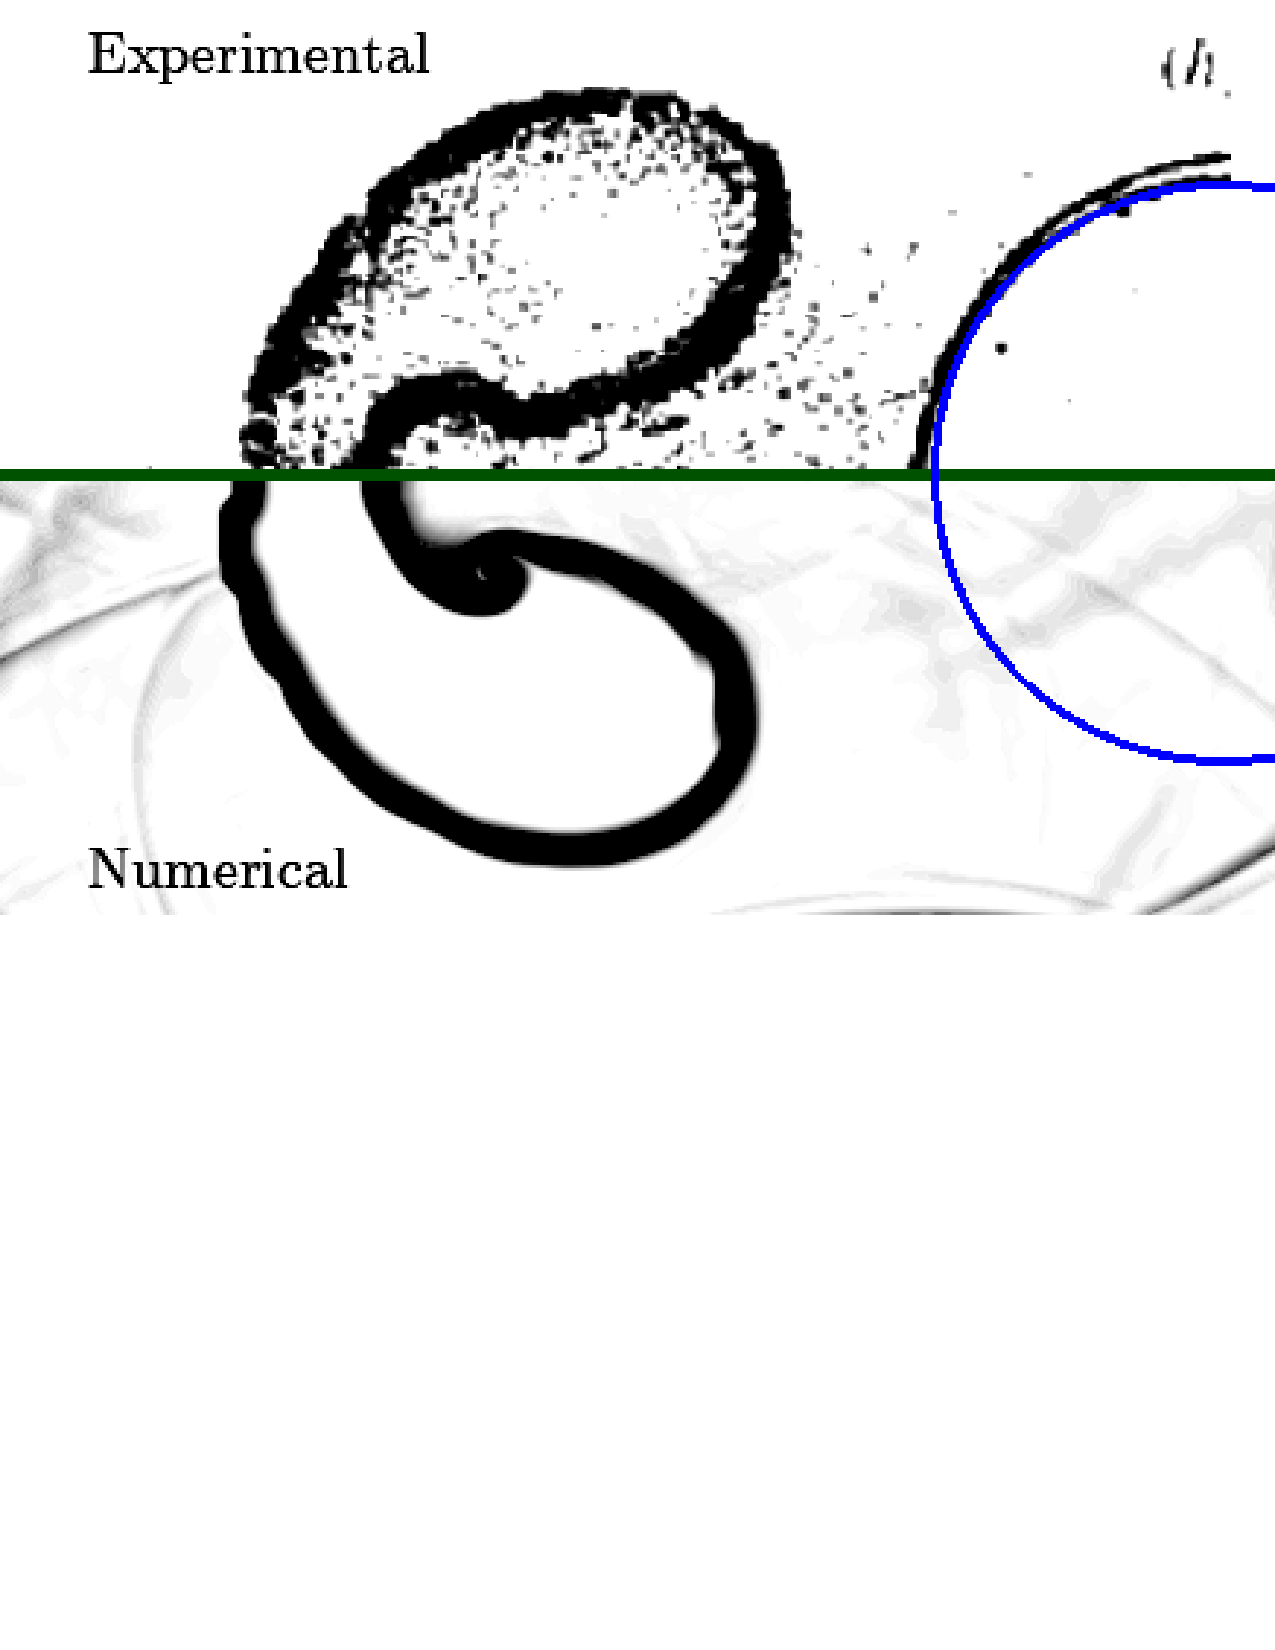
\includegraphics[width=0.3\linewidth]{results/helium_cropped.pdf} % Adjust the path and size
%	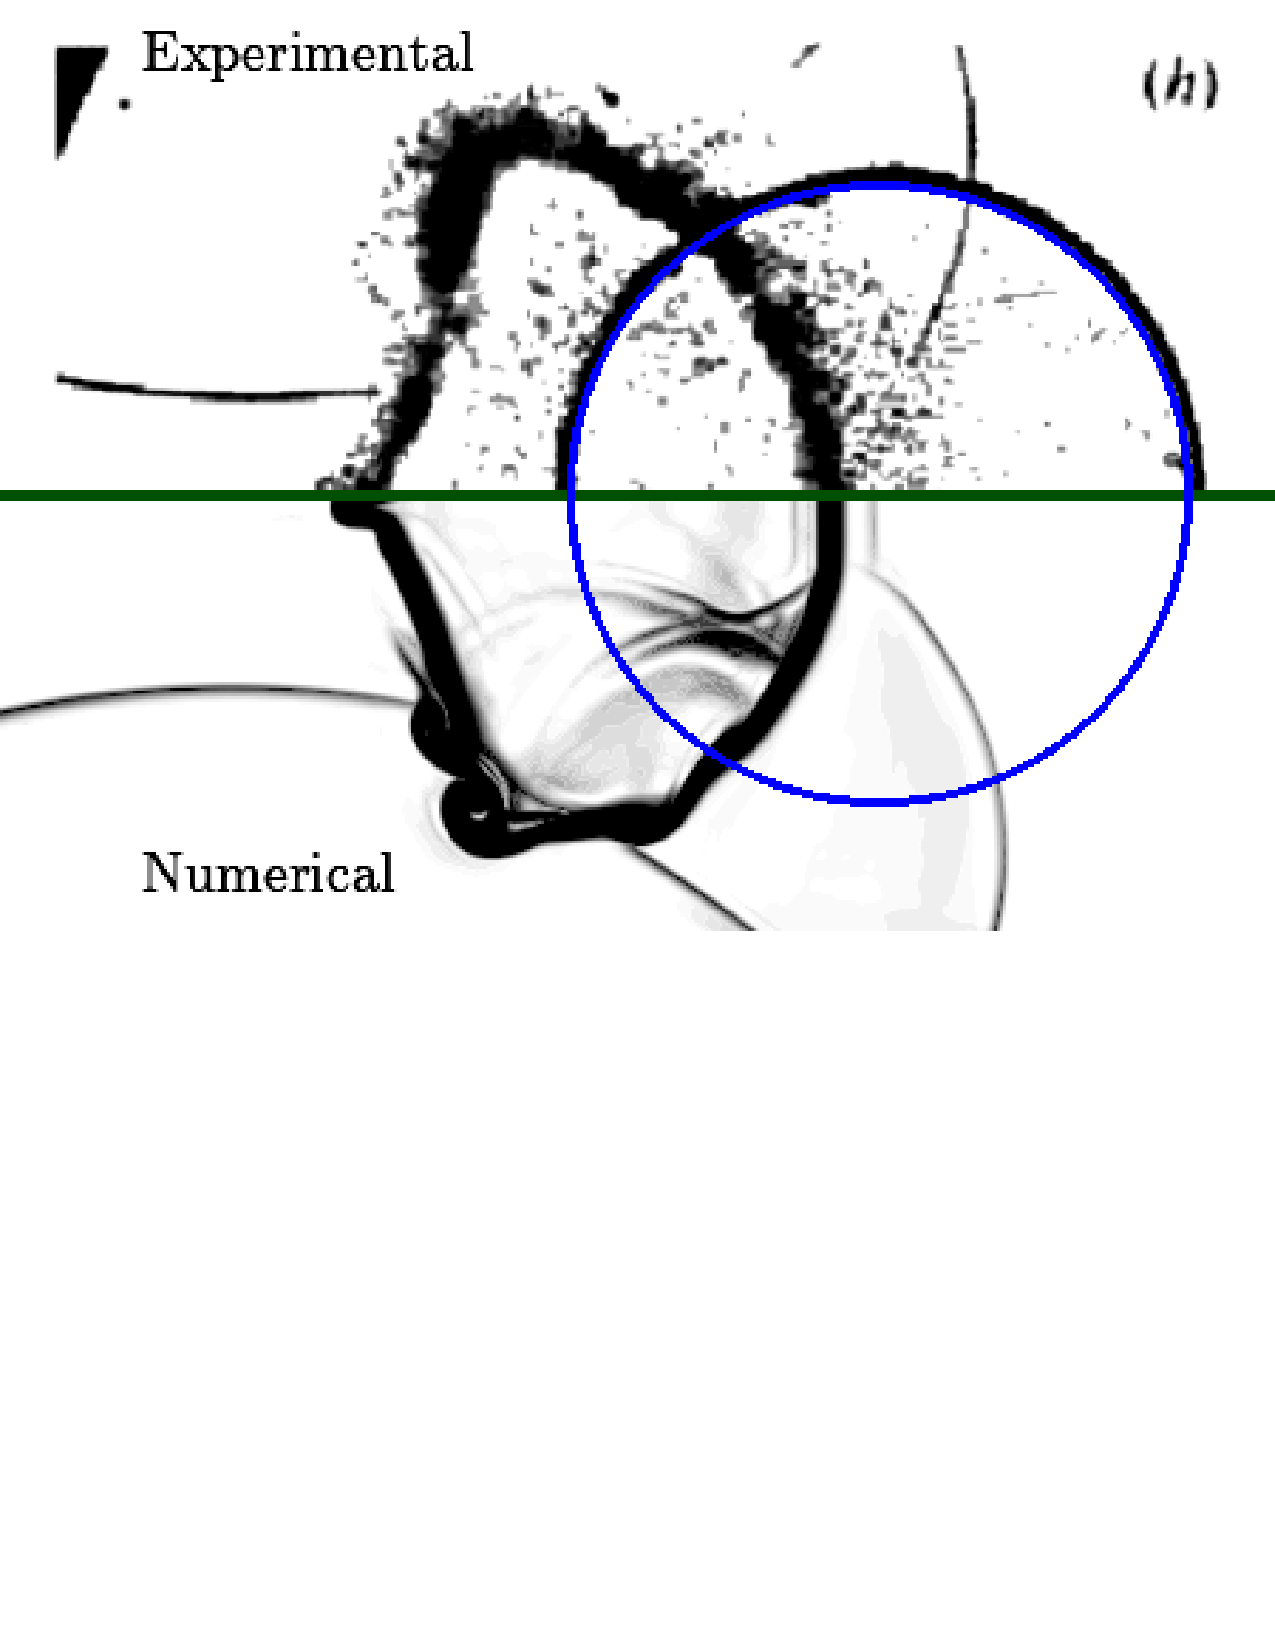
\includegraphics[width=0.3\linewidth]{results/r22_cropped.pdf} % Adjust the path and size



\end{frame}


\begin{frame}{Shock--Bubble Interaction}
	\centering
	\begin{minipage}[t]{0.62\textwidth}
		\centering
		\textbf{Helium} % Display the caption as bold text
		% First set of images
		\foreach \index in {1, ..., 31} {
			\only<\index>{ % Display only the current index
				\includegraphics[width=1.0\textwidth]{results/simulation_frames_helium/frame_\index.png}
				\vspace{0.5em} % Add vertical space between images
				}
			}
			%Trick
			\only<32>{ % Display only the current index
				\includegraphics[width=1.0\textwidth]{results/simulation_frames_helium/frame_31.png}
				\vspace{0.5em} % Add vertical space between images
			}
	\end{minipage}    
	\\ % Add horizontal space between minipages
	\begin{minipage}[t]{0.62\textwidth}
		\centering
		\textbf{R-22} % Display the caption as bold text
		% Second set of images
		\foreach \index in {1, ..., 31} {
			\only<\index>{ % Display only the current index
				\includegraphics[width=1.0\textwidth]{results/simulation_frames_r22/frame_\index.png}
				\vspace{0.5em} % Add vertical space between images
				}
			}
			\only<32>{ % Display only the current index
				\includegraphics[width=1.0\textwidth]{results/simulation_frames_r22/frame_31.png}
				\vspace{0.5em} % Add vertical space between images
			}
	\end{minipage}    
\end{frame}


\begin{frame}{Shock--Bubble Interaction\footnote{{\tiny J.-F. Haas, B. Sturtevant, 1987, Interaction of weak shock waves with cylindrical and spherical gas inhomogeneities.}}}
\centering

\begin{figure}[h]
	\centering
	\begin{subfigure}{0.45\linewidth}
		\centering
		\caption*{\textbf{Helium}}
		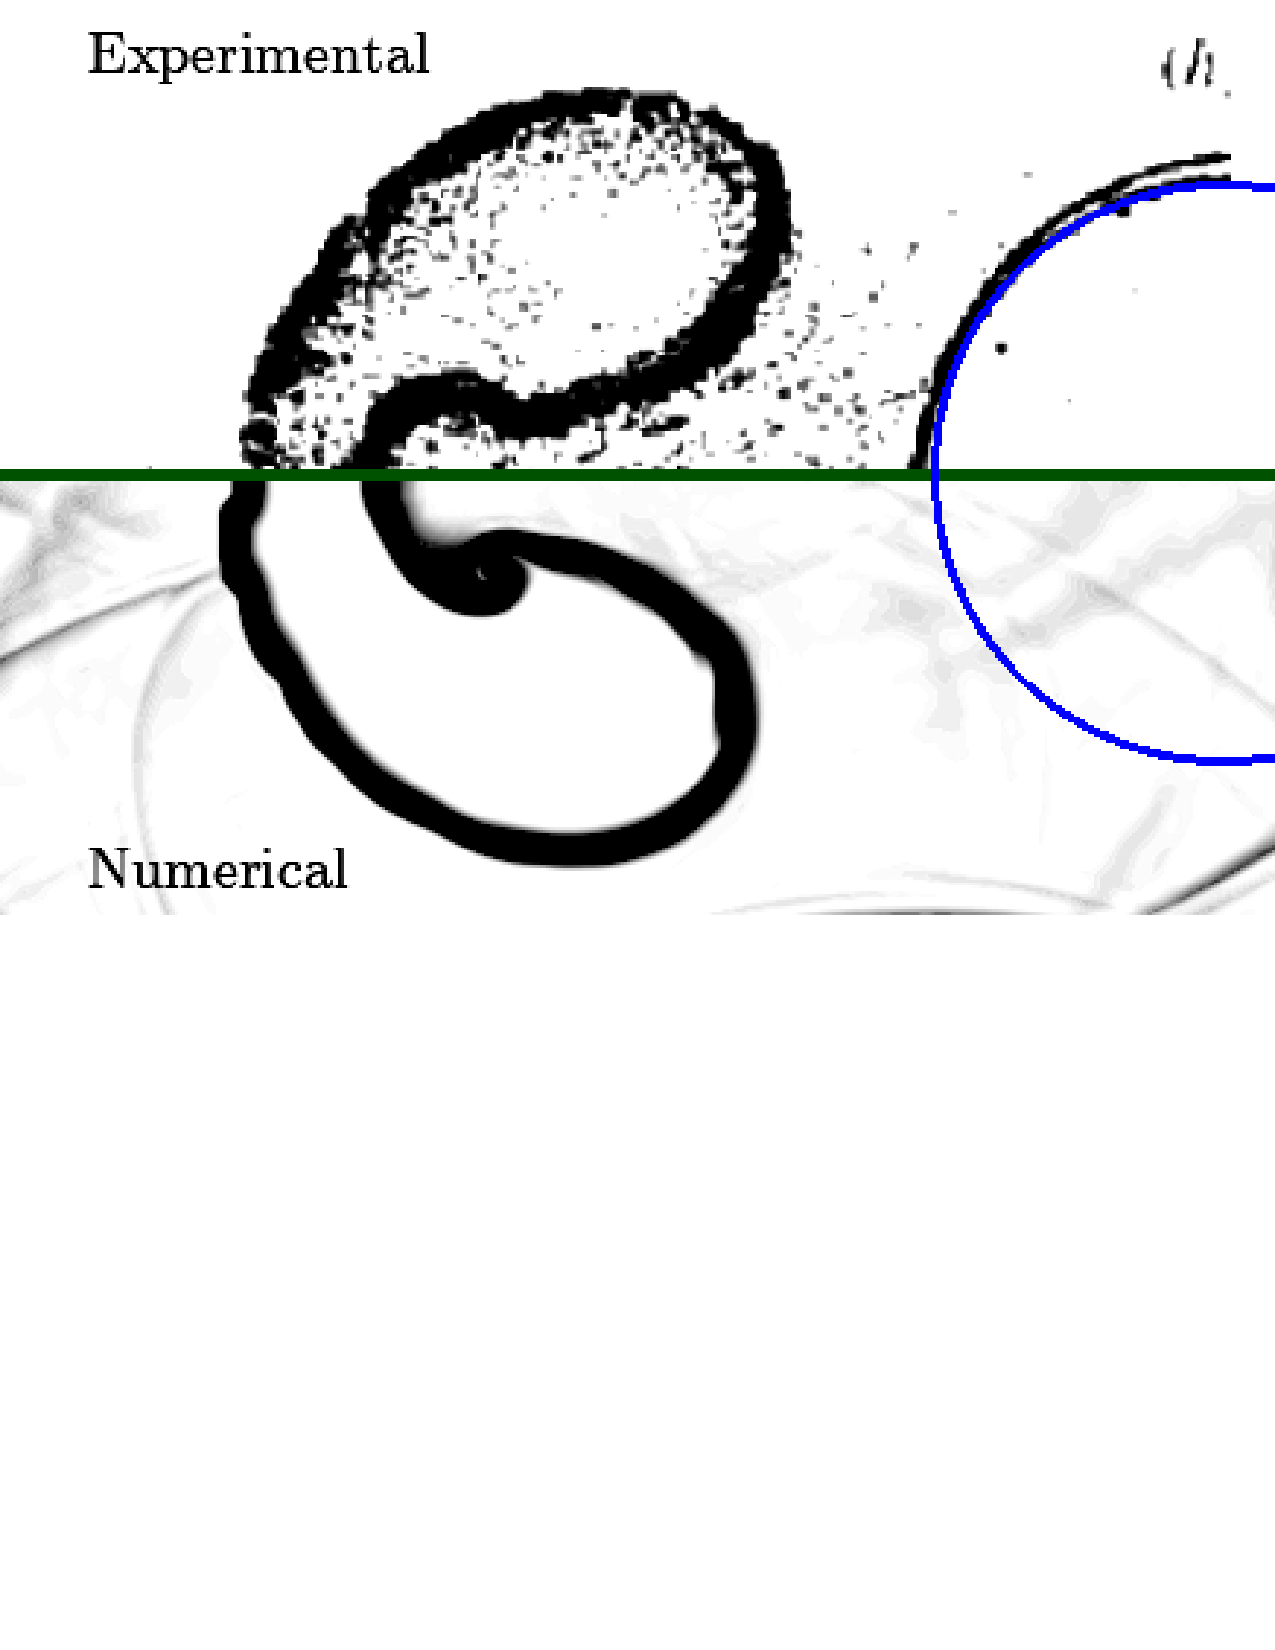
\includegraphics[width=\linewidth]{results/helium_cropped.pdf} % Adjust the path and size
	\end{subfigure}\hspace{1em} % Horizontal spacing
	\begin{subfigure}{0.45\linewidth}
		\centering
		\caption*{\textbf{R-22}}
		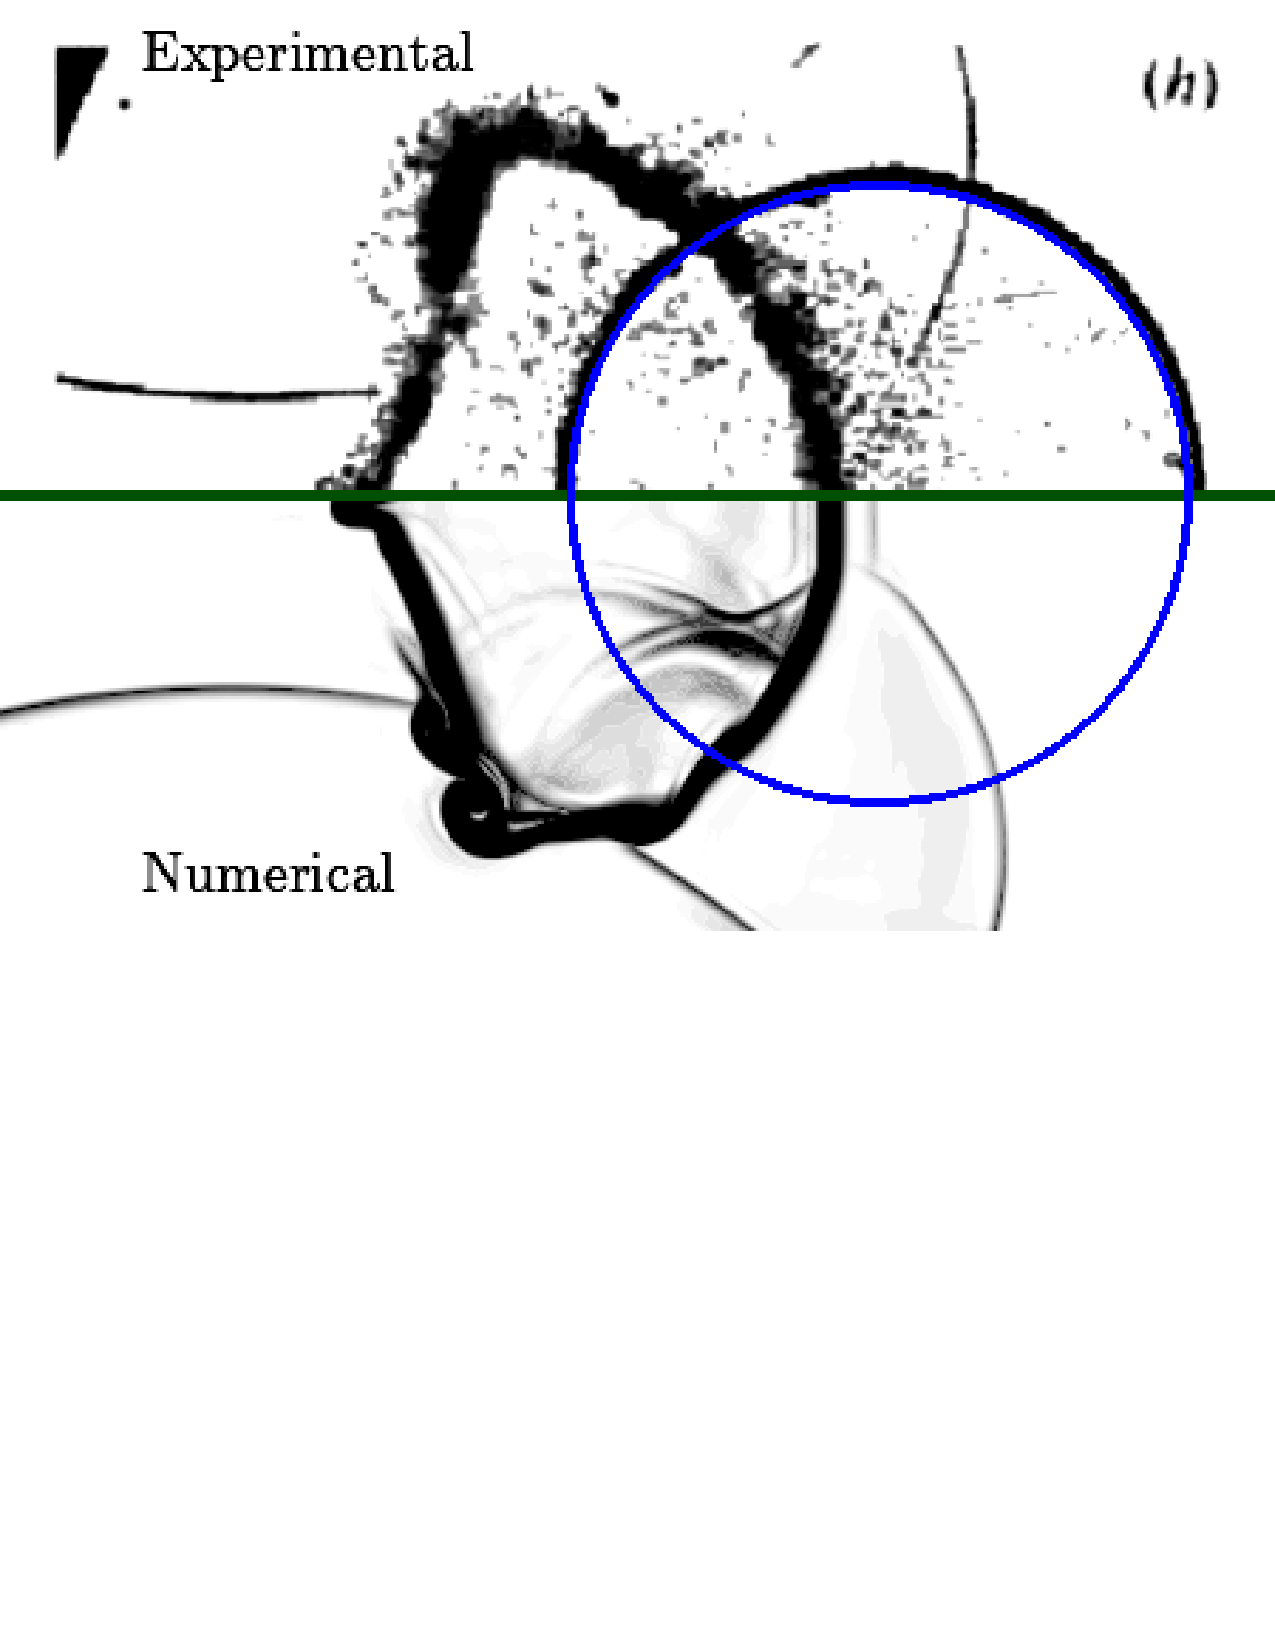
\includegraphics[width=\linewidth]{results/r22_cropped.pdf} % Adjust the path and size
	\end{subfigure}
\end{figure}

\vspace{-7em}

\end{frame}




\setbeamercolor{frametitle}{bg=BBB,  fg=white}  % Original Frame title background and text color
\setbeamercolor{block title}{bg=white, fg=white}  % Original Block title background and text color


\begin{frame}[label=THEEND]
\frametitle{The End}

\centering Thank you


\end{frame}

\section*{Backup slides}




\end{document}

